\chapter{Scripts de avaliação}
\minitoc

A ideia de usar scripts auxiliares prende-se com o facto de muitas pequenas operações conseguem ser muito simplificadas com a rápida implementação
de um script que ajue a resolver o problema em questão. Como linguagem principal usamos essencialmente o \textrm{Perl} por ser uma linguagem fundamental para esta \textrm{UCE},
mas porque também estarmos satisfeitos com as potencialidades únicas que apresenta.\\
Algumas vezes deparámos-nos com pequenos problemas onde não se justifica o uso de \textrm{Ruby} ou \textrm{Haskell} por trazer mais complexidade e baixar o ritmo ao
desenvolvimento desta aplicação.

\section{Geração de imagens}\label{sec geraimg}
Foi desenvolvido um script que usa essencialmente o módulo \textrm{GD} do \textrm{Perl} para gerar estatisticas relativas ao número de linhas do projecto submetido.
Este script (count.pl) encontra-se muito bem documentado, acompanhado de um \textrm{README} onde é explicado o seu funcionamento:

\begin{code_files}
perl count.pl -open <dirPath> [-verbose] [-separated | -allTogether]
    [-percent] [-bars | -pie] -out <fileNamePrefix>
\end{code_files}

Este script na sua utilização minima pode ser executado da seguinte maneira:
\begin{code_files}
perl count.pl -open ~/projecto -out projecto
\end{code_files}

Isto irá pesquizar recursivamente na pasta \textrm{\textasciitilde{}/projecto} todos os ficheiros de várias linguagens de programação e produzir $3$ imagens, todas elas com o
prefixo \textrm{projecto}.

\begin{code_files}
projecto_LinesPerLanguage.png
projecto_FilesPerLanguage.png
projecto_RatioFilesLines.png
\end{code_files}

Cada uma destas $3$ imagens contem informação relativa à totalidade do projecto, a primeira imagem (\ref{fig:linesperlanguage}) mostra a quantidade de linhas
de código e de comentários relativamente a todas as linguagens presentes no projecto. Desta forma conseguimos ter uma noção do impacto que cada linguagem
tem para o projecto final e a quantidade de documentação que existe relativamente a cada linguagem.

\begin{figure}[htbp]
\begin{center}
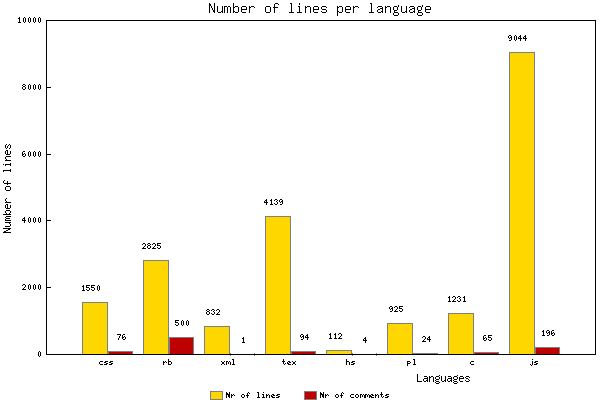
\includegraphics[width=0.9\textwidth]{Images/projecto_LinesPerLanguage.png}
\caption{Linhas por Linguagem}\label{fig:linesperlanguage}
\end{center}
\end{figure}

Outra imagem que a execução do comando anterior gera é a quantidade de ficheiros por linguagem, assim sendo temos uma noção da modularidade que existe
em cada utilização de cada uma das linguagens utilizadas.

\begin{figure}[htbp]
\begin{center}
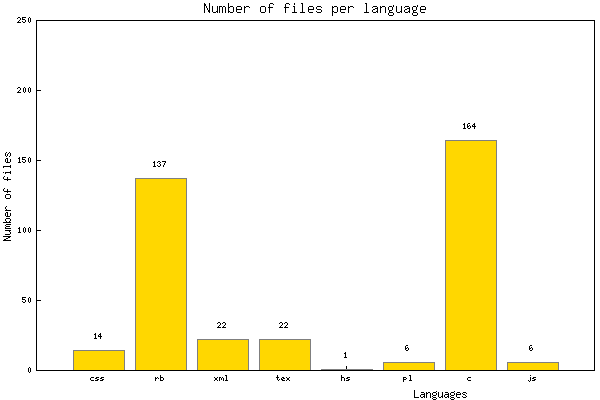
\includegraphics[width=0.9\textwidth]{Images/projecto_FilesPerLanguage.png}
\caption{Ficheiros por Linguagem}\label{fig:filesperlanguage}
\end{center}
\end{figure}

A última imagem gerada é um rácio entre o número de ficheiros e o número de linhas para cada linguagem. Assim conseguimos ter uma
noção do número médio de
linhas que constituí cada um dos ficheiros do projecto.

\begin{figure}[htbp]
\begin{center}
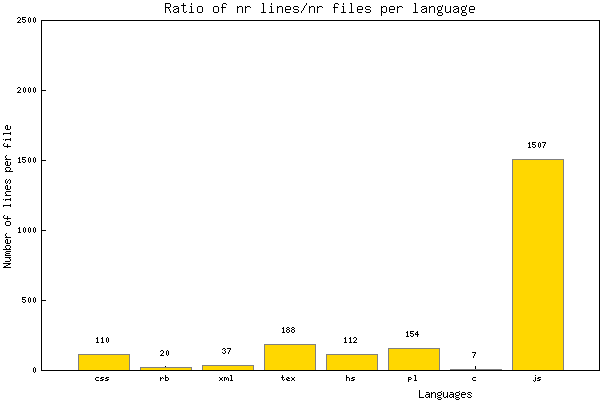
\includegraphics[width=0.9\textwidth]{Images/projecto_RatioFilesLines.png}
\caption{Linhas por Linguagem}\label{fig:ratiofileslines}
\end{center}
\end{figure}

Como se pode verificar, todas estas estatísticas são meramente um indicador e nada de maior se pode concluir, sem ser apenas ter uma
noção global da quantidade de linhas
e o uso de quais linguagens relativamente a um projecto.

Caso queiramos podemos ainda gerar as mesmas imagens, mas em percentagem. Como é obvio não faz sentido gerar percentagens
sobre rácios, assim quando o utilizador
emite o comando:

\begin{code_files}
perl count.pl -open ~/projecto -out projecto -percent
\end{code_files}

geramos apenas a percentagem para as duas primeiras imagens.\\

Uma outra utilização interessante deste script permite a geraçã de uma única imagem com o intuíto de ter um resumo de todo o projecto
submetido numa única imagem, como
se a imagem que sumariza a utilização de linhas do projecto.\\
Para gerar este ficheiro precisamos de fazer:
\begin{code_files}
perl count.pl -open ~/projecto -out projecto -all
\end{code_files}
Por defeito quando utilizamos esta flag, todos os resultados que vão aparecer irão ser em percentagem, visto que podemos ter uma
grande disparidade de números de
linhas entre várias linguagens. Obtemos assim a imagem \ref{fig:projectlanguages}:

\begin{figure}[htbp]
\begin{center}
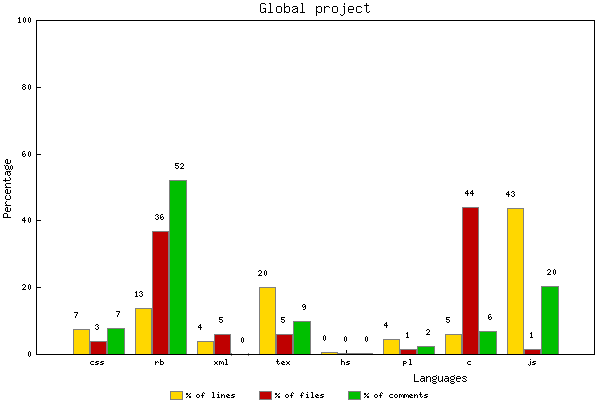
\includegraphics[width=0.9\textwidth]{Images/projecto_projectLanguages.png}
\caption{Visão global do projecto}\label{fig:projectlanguages}
\end{center}
\end{figure}

Este script é ainda capaz de gerar pie charts em vez de gráficos de barras.

\section{Makefile}
O nosso sistema de submissão permite ao utilizador submeter um \textrm{makefile} afim de facilitar a compilação do código do seu
projecto, caso a compilação deste seja mais
exigente do que uma trivial passagem pelo \textrm{gcc}. Assim é necessário extrair do \textrm{makefile} a informação sobre o ficheiro
objecto que este vai gerar aquando da
execução do comando \textrm{make}.\\
Servindo-nos do módulo \textrm{Perl} \textrm{Makefile::Parser} conseguimos, com poucas linhas extraír o nome do binário que irá ser
gerado pelo \textrm{makefile}.\\

Muitas das vezes, são scripts com a simplicidade que este apresenta que fazem a diferença e que mostram o verdadeiro poder de estar à
vontade numa linguagem de utilização rápida como sao as de scripting e nomeadamente o \textrm{Perl}.\\

Pretendemos melhorar este script e não o damos como terminado.
\section{Cloning}
Um dos objectivos finais para este projecto é que o sistema tenha um mecanismo de detecção de clones.\\
Apesar de ainda não implementado no sistema, o nosso trabalho nesse sentido já começou. Criamos um script na linguagem \textit{Perl},
a linguagem escolhida prende-se com o facto de grande parte das tarefas realizadas pelo script serem de processamento de texto.\\
De seguida vamos descrever passo a passo o que o script faz actualmente, tendo em conta que ainda não está preparado para ser
utilizado no sistema:\\
\begin{itemize}
\item recebe um ficheiro por parâmetro
\item executa o comando \textit{ctags -x *.c}, cujo output contém entre outras coisas, o nome das funções que existem nos ficheiros c
encontrados, e as linhas referentes a cada um
\item a partir do output do ctags retira as linhas que identificam o ínicio de cada função
\item lê o ficheiro recebido como parâmetro, divide-o por funções, guardando as linhas de cada uma, numa posição da hash
\item analisa cada posição da hash e altera-a, retirando todos os comentários e espaços, substituíndo todas as variáveis por \textit{var},
todas as strings por \textit{S} e todos os números por 1
\item de seguida lê um segundo ficheiro e trata-o da mesma forma que o primeiro
\item por fim compara cada posição da primeira hash com todas as posições da segunda. Se houver casos em que as duas são iguais,
imprime para o STDOUT um aviso
\end{itemize}

Temos noção de que o script precisa de algumas reformulações para a sua integração com o sistema. Para começar, em vez de receber
apenas um ficheiro por parâmetro deverá receber o path de dois ficheiros. Além de preparamos o script para ser integrado no sistema 
também é necessário afiná-lo de modo aque não existam muitos falsos positivos.\\
Estas entre outras, serão algumas das alterações ao script feitas para a próxima fase, que garantirá ao sistema a ferramenta necessária
para a detecção de clones.







